\documentclass[twocolumn]{article}
\usepackage[utf8]{inputenc}
\usepackage[english]{babel}
\usepackage{lipsum}
\usepackage{multicol}
\usepackage{abstract} % Allows abstract customization
\usepackage{footnote}
\usepackage{listings}
\usepackage{url}
\usepackage{dblfnote}
\usepackage{graphicx}
\usepackage[margin=1in]{geometry}
\usepackage{cite}
\usepackage{natbib}
\usepackage{amsmath}
\usepackage{algorithm}
\usepackage[noend]{algpseudocode}
\usepackage[]{units}

\graphicspath{ {images/} }
\bibliographystyle{apj} 
\setlength{\columnsep}{1cm}

\makeatletter
\def\BState{\State\hskip-\ALG@thistlm}
\makeatother



\begin{document}

\twocolumn[\begin{@twocolumnfalse}
  \centerline{\Large\bfseries Simulation of Stellar Streams Within the Milky Way}
  \vspace{3ex}
  \centerline{Peixian Wang}
  \centerline{May 6, 2016}
  \vspace{3ex}
  
  \begin{abstract}
		 We study the dynamics of satellite galaxy structures around the Milky Way, which is host to various satellites of unique masses. We use NEMO as a base code to model $N$-body simulations for satellites around a circular orbit centered on the Milky Way, with various initial masses. We find that the shape and length of the stellar stream heavily depends on the initial satellite mass. 
  \end{abstract}
   \vspace{3ex}
\end{@twocolumnfalse}]

\section{Introduction}

The Milky Way's vast arrangement of stars is broadly categorized into three components: the disk, the bulge, and the halo. However, over the past two decades surveys have uncovered more aspects of the Milky Way, particularly regarding the rings composed of stars, gas, and dust around the Milky Way, known as stellar streams. 

We investigate shape of the stellar streams as a result of varying progenitor masses, with this paper organized as follows: in section 1, we detail the discover, formation, and visible structure of stellar streams, as well as providing examples of nearby stellar streams. In section 2, we describe the initial conditions and various methods needed to set up a stellar stream simulation. Section 3 introduces NEMO, a stellar dynamics toolbox framework we used to simulate various stellar streams. Section 4 describes in detail one simulation in particular, while section 5 details the results of all simulations. Finally, in section 6 we present our conclusions, compare to other works, and describe additional research to be conducted.

\subsection{Discovery}

In the early 1970's, surveys of the Cartwheel galaxy (ESO 350-40) lead to predictions that its rings could be a result of galaxy mergers, shown in figure \ref{fig:cartwheel}. \cite{lyndsAndToomre} verified these predictions by matching the mass dispersion of the rings to a kinematic epicyclic oscillations model after an impulsive disturbance occurs, showing that there was a strong likelihood that Cartwheel galaxy's rings were created through galactic mergers. 


Since then, a multidude of observed examples have been found, with the most popular examples being NGC 4013. An edge-on barred spiral galaxy within the constellation Ursa Major, a survey conducted by \cite{delgado} found a stellar stream stretching over 80 thousand light-years from the galactic center. Figure \ref{fig:ngc4013} shows an overlay of the H I contours onto an image of NGC 4013, with a noticeable H I gas warp within the top left region.

\begin{figure}
	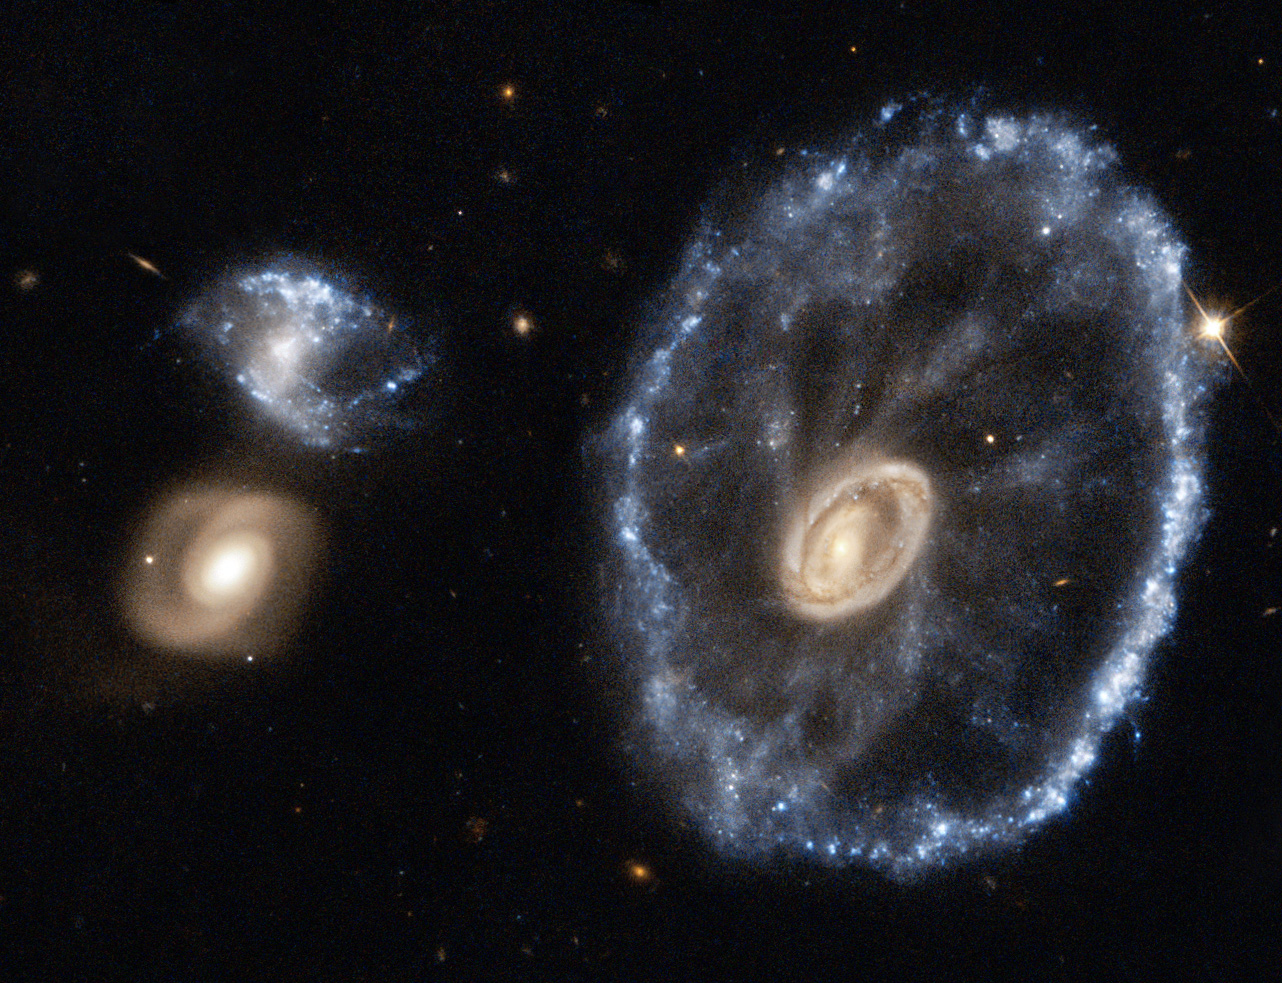
\includegraphics[width=8cm]{cartwheel.jpg}

	\caption{Cartwheel Galaxy, \cite{cartwheel}}
	\label{fig:cartwheel}
\end{figure}

\begin{figure}
	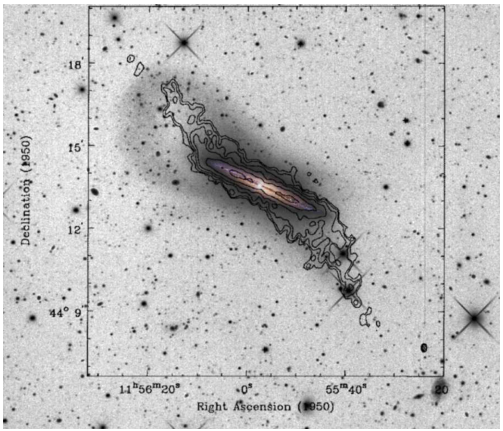
\includegraphics[width=8cm]{h1Contours.png}
	\caption{H I Contours of NGC 4013, showing the stellar stream wrapping around a large HI cloud in the top right. From \cite{delgado}. }
	\label{fig:ngc4013}
\end{figure}

NGC 4651 is another often cited example of stellar streams, as it contains a particularly eccentric stellar stream. After N-body simulations conducted by \cite{foster}, it was found that the stellar stream was created due to tidal disruption of a dwarf satellite originally on a very eccentric orbit, showin in figure \ref{fig:ngc4651}


\begin{figure*}
	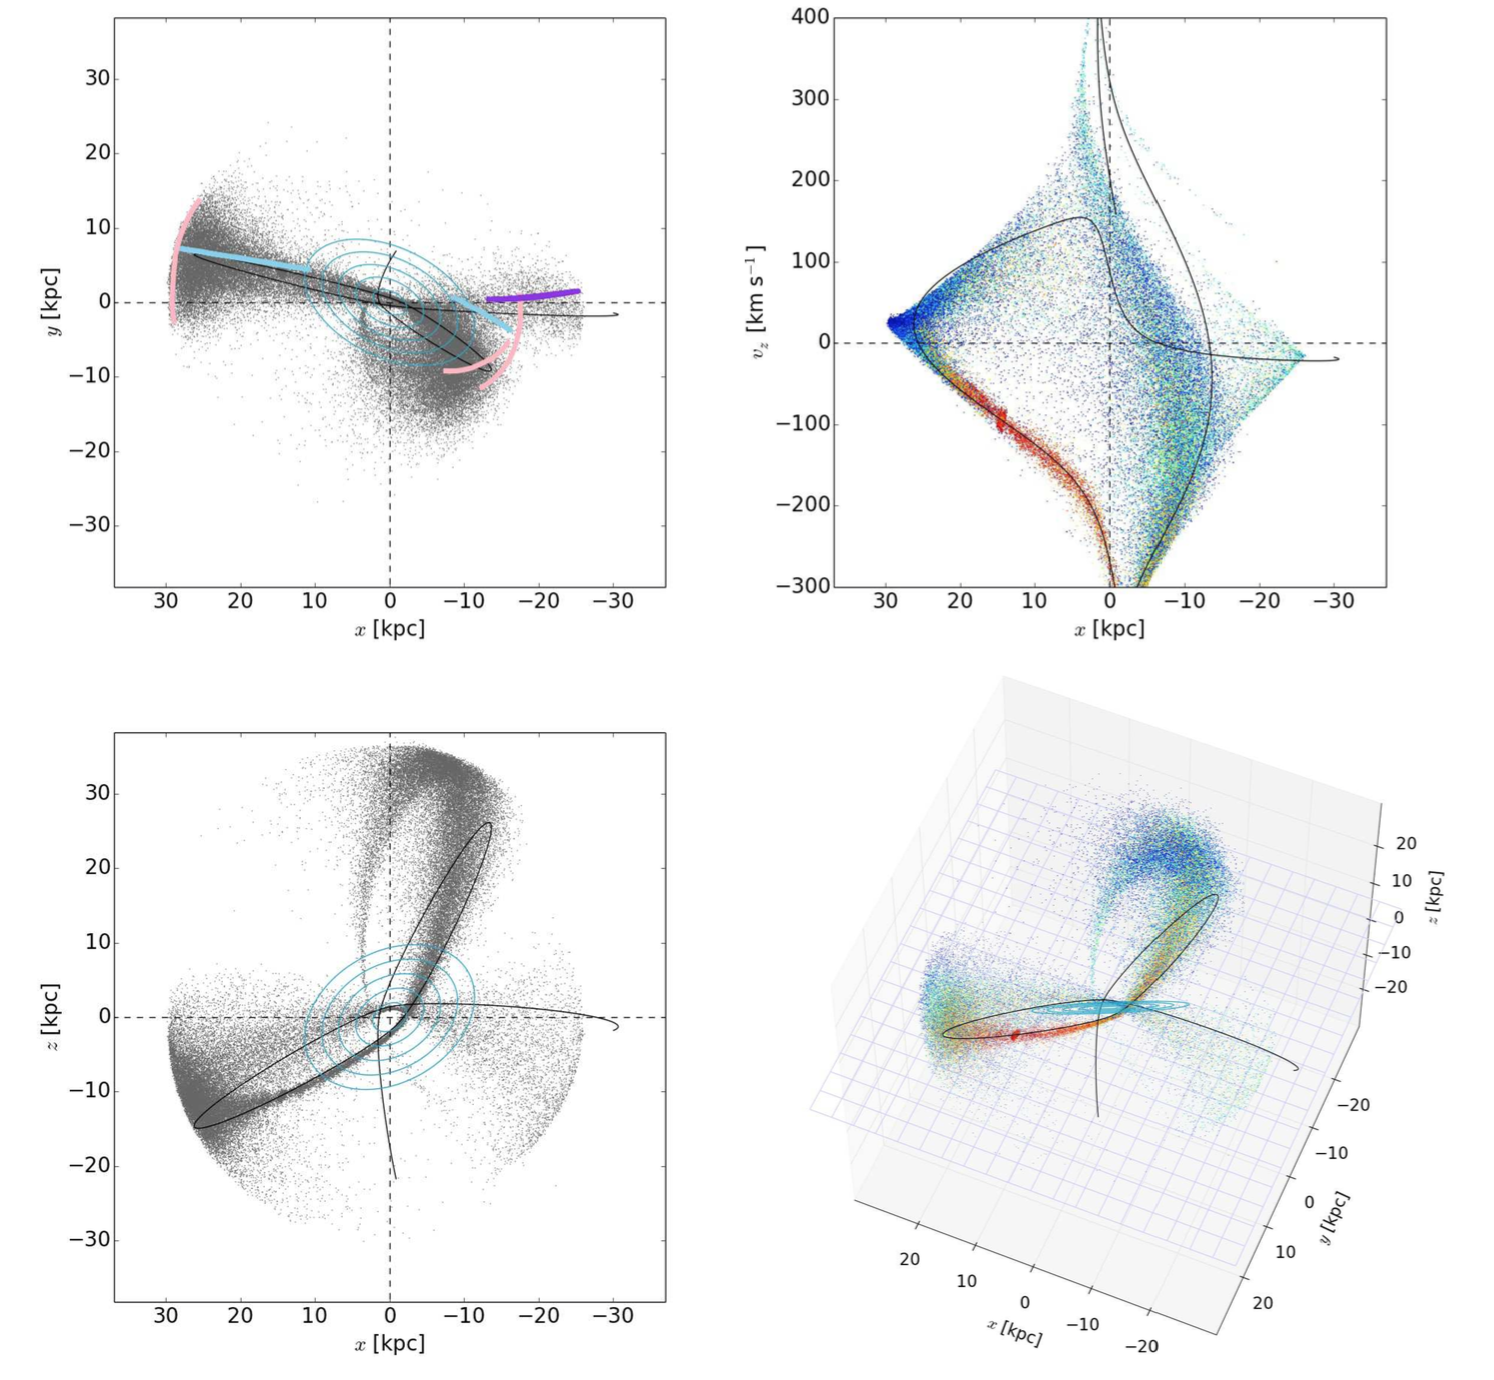
\includegraphics[width=\textwidth]{nbody-umbrella.png}
	\caption{\textit{N}-body simulations of an NGC 4651-type stream. Small dots correspond to \textit{N}-body particles, black curves represent the inferred orbit of the progenitor dwarf satellite galaxy, and light blue ellipses are the stellar disc in spacings of one disk scale-length. Upper-left panel shows the $x, y$ positions on the sky, with colored curves corresponding to the various features. Upper-right panel shows a position-velocity phase-space diagram where the particles are color-coded by initial binding energy within the progenitor satellite (red for most bound, blue for least bound). The lower-left panelis an orthogonal projection to the sky so that line-of-sight distances $z$ are visible, the remnant of the progenitor nucleus is seen as a clump on the near side of the galaxy. The lower-right panel shows a tilted view to illustrate the trajectory of the stream relative to the disk; the stream passes through the galaxy at small radii on one side, and at a large radius on the other. From \cite{foster}. 
	\label{fig:ngc4651}
	}
\end{figure*}

The observed streams in other galaxies are often visible because of how bright the streams are relative to their surroundings. 
Since the orbits of all celestial objects are affected by some form of orbital resonance, stellar streams find themselves no exception. Within the region in which the resonances occur, the collision of gas clouds excite star formation, causing this region to be extremely bright. By using the inverse of this relationship, \cite{ringsAndPseudoRings} found galactic resonances using rings and pseudorings. Since fine grain IIIa-J emulsion makes it possible to spot the faint and small stellar streams, it was found that the stellar streams orbiting over 1000 early to intermediate Hubble type spiral galaxies within the southern hemisphere do follow the Linblad resonance. From this, it becomes possible to infer the rough orbits of possible galaxies that lie within the resonances. 

A subset of these stellar streams are polar rings, which similarly consist of dust, stars, and gas. NGC 660 is a popular example, with its polar rings roughly aligned in its minor axis. These minor polar rings are found to consist of mostly neutral hydrogen, along with a ratio of velocity distribution from the central bulge to the circular velocity being abnormally high (\cite{distributionOfAtomicHydrogen}). These polar rings also contained blue stars and several billions of solar masses in gas, despite the gas-deprived host galaxy, suggesting that the polar rings were also formed by accretion or cannibalization from other companions relatively recently. The shape of the polar rings are curious however, since the tilted structure, relative flatness, and precession speed all suggest that the shape of the polar ring should be not exist than a Hubble time (\cite{selfGravitatingPolarRings}). Yet the existence of some polar rings that maintain their shape but also contain redder stars refute this notion, thereby suggesting that somehow the rings themselves have settled, or forced into settling, into a stable equilibria with the gravitational field. \cite{symmetricStellarRings} found that a quasi-impulsive kinematic oscillation equations provide accurate models into the ring structure and a $N$-body simulation is sufficient to model the shape and dynamics of these rings. 

\subsection{Composition \& Formation} 
$N$-body simulations have previously strongly suggested that the galactic merging of smaller galaxies is a main cause for galaxy formation, as found by\cite{galaxyNBody}, which strongly suggest that stellar streams are a result galaxy's galactic tide cannibalizing on nearby satellite galaxies. This mechanism only affects the satellite galaxy due to the relatively weak gravitational fields, but by using fossil signature of ancient accretion events within the Milky Way halo, \cite{accretionEvents} found that if the satellite galaxy is very small, the debris trails remain aligned to the parent satellite galaxy's orbit, for the lifetime of the host galaxy. These orbits become extremely close to circular once the orbit is near planar. If the mass of the satellite galaxy is greater than one ten-thousandth of the host galaxy, then the stellar stream produced in the process has two non-equidistant trailing points where the attractive force of the host halo and satellite are at zero-velocity. As a result of this, \cite{dynamicsOfTidalTails} postulated that a stellar stream that is created begins to be affected by the satellite's own self-gravity, and thus begins to be accelerated into many different directions. These directions vary based on the mass of the satellite and host, along with the structure of the halo. Due to this, the radial velocity of stars left in the stellar stream will vary proportionally to the satellite galaxy's mass, which then means that all models for stellar streams would need to be mass-dependent modeling. 

\subsection{Structure}
A stellar stream is a two-tailed system, composed of a leading tail and a trailing tail (sometimes called a leading arm and a trailing arm). The leading tail is characterized by a gradual fall into the host galaxy's center, while the trailing tail is characterized by a spiral outward. Figure \ref{fig:sagittarius3d} shows a projection the Sagittarius stream around the Milky Way, displaying the visible structure of the leading and trailing tails. 

\begin{figure}
	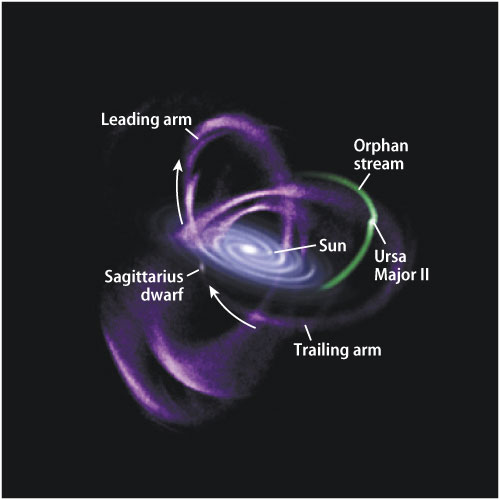
\includegraphics[width=8cm]{sag_3d.jpg}
	\caption{Rendition of the Sagittarius Stream, \cite{fieldOfStreams}}
	\label{fig:sagittarius3d}
\end{figure}

\subsection{Stellar Streams within the Milky Way} 

\subsubsection{General Properties} 

\begin{figure*}
	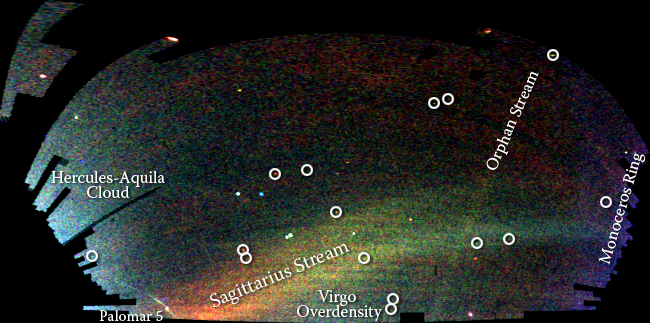
\includegraphics[width=\textwidth]{fieldofstreams.jpg}
	\caption{Vasily's Field of Streams, \cite{fieldOfStreams}}
	\label{fig:fieldOfStreams}
\end{figure*}

As this paper focuses mainly on stellar streams created with Milky Way and Milky Way satellite galaxy conditions, we will focus the bulk of the information on these conditions. In 2002, a peculiar group of F/G stars with $B-V \leq 0.7$ and $V$-band apparent magnitudes in the range 17.0-19.5 were found between 30$^\circ$ above and 45$^\circ$ below the Galactic plane, spanning a distance of 5 kpc \cite{lastMajorInvasion}. These stars had a mean rotation speed of ~\unitfrac[100]{km}{s}, \unitfrac[80]{km}{s} off from the predicted ~\unitfrac[180]{km}{s}. Retaining kinematic signatures that distinguish themselves from the other stars within the think disk. This group of stars were identifiable due to the asymmetry in the number of stars in the thin disk and inner halo on one side of the galactic center. As a result this group of stars was theorized to be a result of the a satellite galaxy that merged with the Milky Way, possibly forming the thick disk in the process. This process also led to conclusions that stars within stellar streams would be distributed with lower net rotational streaming than the rest of the disk. The same kinematic signatures can be applied in a similar manner to the halo, many moving groups and halo substructures have been found with relatively similar kinematic signatures, suggesting that the halo was similarly affected by the satellite galaxies. 

The idea of satellite galaxies interacting with the Milky Way in a non-trivial way is not foreign either: the orbital path of the Sagittarius dwarf spheroidal galaxy is highly correlated with at least four of the globular clusters within close proximity to the Milky Way. These four globular clusters are distributed along the path of the Sagittarius Stream, along with the observational evidence that stars within the Sagittarius galaxy are being lost to the Milky Way due to the Milky Way's tidal force, led to conclusions that these four clusters were originally former members of the Sagittarius galaxy (\cite{globlarClusters}).

\subsubsection{Virgo Overdensity \& the Sagittarius Stream} The Virgo overdensity and Sagittarius Stream are given special attention due to their secularity and uniqueness. Found in 2000 by  \cite{ghostOfSagittarius} using accurate multi-color Sloan Digital Sky Survey (SDSS) by probing structures in the Milky Way halo with distances in the range of 2-150 kpc, two branches of the Sagittarius stream were found, with stars having significantly bluer turnoff. Since the Sagittarius galaxy has an orbital path that is high inclined with respect to the disk inclination, it crosses the Milky Way near the Virgo constellation. 

A survey conducted by \cite{virgoOverdensity} found that the Virgo constellation hosts a clump of 21 RR Lyrae stars (henceforth referred to as the Virgo overdensity, shown in figure \ref{fig:fieldOfStreams}) which has a considerably smaller line of sight depth than the RR Lyrae overdensity at the epicenter of the Sagittarius stream. Following the construction of a three-dimensional density distribution, the Virgo overdensity shows a giant clump of stars crossing the Galactic plane orthogonally and even extending into the souther Galactic hemisphere. Martinez-Delgado et al, through a $N$-body simulation of one of the arms belonging to the Sagittarius galaxy, found that the properties of the Virgo overdensity matches the theoretical models of the Sagittarius stream, suggesting that the Virgo overdensity is actually an arm of the Sagittarius galaxy falling into the Milky Way disk. 

\subsubsection{Other Streams within the Milky Way}
Beyond the Sagittarius stream, many other streams exist within the Milky Way, with notable ones such as the Arcturus Stream, Magellanic Stream, and Monoceros ring. Near the star Arcturus, the Arcturus Stream was found as a result of similar proper motion, containing older stars lacking in heavy elements surveyed by \cite{ghostOfSagittarius}. The Magellanic Stream consists of large gas clouds, first found in 1965. Stretching to over 180 kpc, the gas was observed to be moving extremely fast by \cite{magellanicStream}. The Monoceros Ring is a result of the Canis Major overdensity, a ring spanning over 200,000 light years, wrapping around the Milky Way over three times, as observed by \cite{monocerosRing}, shown in figure \ref{fig:fieldOfStreams}. 

\subsection{Research Potential \& Impact}
Research in stellar streams lends a great amount of insight into the early formation of galaxies. For example, the Sagittarius stream crosses the Milky Way twice in a particular bifurcation, shown in figure \ref{fig:sagittarius3d} and \ref{fig:fieldOfStreams}. This particular bifurcation shape lead to various simulations from \cite{sagittariusFork}, who then found that the only way such a bifurcation could occur would be to have the Milky Way's dark matter halo as a round spherical. At that time, the Milky Way halo was considered to be a flattened spheroidal, which meant that the Sagittarius Stream's bifurcation lead to an insight on the structure of the Milky Way halo. Due to this discovery, further simulations of stellar streams can indicate the status of various satellite galaxies under tidal force. 

\section{Initial Conditions and Methods}
By assuming the base cosmology is a cold dark matter (CDM) cosmology, we can then further make the assumption that dark matter halos have a universal density profile, which is the same assumption made by \cite{dynamicsOfTidalTails}. This can be modeled by equation \ref{eq:rho}:

\begin{equation}
\rho(r) \propto r^{-1}(r+r_s)^{-2}
\label{eq:rho}
\end{equation}  

In equation \ref{eq:rho}, $r_s$ is the scale length based on the virial radius, which can, in turn, then be modeled through equation \ref{eq:nfwProfile}:

\begin{equation}
	R_{virial} = cr_s
	\label{eq:nfwProfile}
\end{equation}

Thus we can start by modeling the Milky Way halo as a static halo potential. A potential problem with a static halo potential is that the effects of dynamical friction are ignored, leading to a possible erroneous simulation. However, \cite{dynamicalFriction} found that the effect of dynamical friction was significant on stars escaping the Milky Way, but only due to the star's near neighbors. Taking into account the density difference between the Milky Way and the satellite galaxies we are trying to model, along with the large distances between the Milky Way and it's satellites, the effects of dynamical friction can be safely ignored to simplify simulations. Furthermore, the effects of dynamical friction only come into significant effect once the stellar stream has formed and has an infall into the Milky Way, and since the purpose of this simulation is to understand the formation of stellar streams, dynamical friction can be safely ignored. 

The satellites can then be modeled with a Navarro-Frenk-White profile, with the outer edge of the halo being the $R_{virial}$, as shown by \cite{bryanNorman}. However, we must also the model the tidal field of the Milky Way for a usable solution, which extends far beyond the $R_{virial}$ of the Milky Way. To fully simulate this takes far more computational power than reasonable, however. The solution to this is to place the satellite already within the tidal field and account for the tidal field change when the satellite is created. 

The satellite halo can thus be modeled as a spherical dark matter halo, and the Milky Way as a point mass, thus ignoring the effects of the Milky Way disk. The satellite halo can be characterized with its initial maximum circular velocity, and then using the acceptance-rejection algorithm each particle within the halo can then be modeled. By setting the concentration parameter as $c = 15$ for the Navarro-Frenk-White profile for both the Milky Way and the satellite, three different sizes of satellites are generated, with the medium size modeled after the Sagittarius Stream. Since the Sagittarius stream is the most obvious and widely recognized stellar stream, it made sense to use it as starting point, with one satellite magnitudes larger and the other satellite magnitudes smaller. Because mass of the stellar streams change continuously as the simulation progresses, it becomes necessary to have an alternate way of measuring satellite size within the simulation, which is the rotational velocity $V_{sat, max}$. Applied to the simulation, we used a 0.45, 0.16, and 0.08 times the maximum rotational velocity for the Milky Way ($V_{mw, max}$) for the rotational velocity, which were the same ones used by \cite{dynamicsOfTidalTails}, and will be henceforth known as Massive, Sagittarius, and Small satellites. The masses are summarized in table \ref{tab:massTable}.

\begin{table*}[t]
	\centering
	\begin{tabular}{| l | l | l | l | }
		\hline Satellite & $M/M_{mw, vir}$ & $R/R_{mw, vir}$ & $V_{max}/V_{mw, max}$ \\ \hline
		Massive & $1.9 \times 10^{-2}$ & $9.02 \times 10^{-2}$ & 0.45 \\ \hline
		Sagittarius & $9.0 \times 10^{-4}$ & $3.38 \times 10^{-2}$ & 0.16 \\ \hline
		Small & $9.9 \times 10^{-5}$ & $1.66 \times 10^{-2}$ & 0.08 \\ \hline
	\end{tabular}
	\caption{Initial mass, radius, and velocity conditions. }
	\label{tab:massTable}
\end{table*}

To fully experiment with the orbital size of each satellite, two different orbits were tested per satellite, with varying eccentricity and apocenters. To properly measure the orbits, the eccentricity was defined through \ref{eq:eccentricity},

\begin{equation}
e \equiv \frac{r_a-r_p}{r_a+r_p}
\label{eq:eccentricity}
\end{equation}

with $r_a$ corresponding to the apocenter and $r_p$ corresponding to the pericenter. Thus two orbits were chosen, with the first being completely circular ($e = 0$) with a radius of $0.4R_{vir}$, and the second having $e = 0.5$, pericenter of $0.2R_{vir}$, and an apocenter of $0.6R_{vir}$. To create the time units, we considered one circular orbital period to be $\approx 2.0$, thus to take 5000 timesteps each timestep was chosen to be $4 \times 10^4$ time units.

% \section{Code Discussion}
% To accomplish this, we decided to use the Enzo, a hybrid hydrodynamics and n-body simulation code. Setting the units where $M_{vir} = 1$, $R_{vir}  = 1$, and the gravitational constant $G = 1$, the galaxy disk problem type in Enzo was used, using the n-body simulation method. In order to apply this into Enzo, we used an adaptive mesh refinement (AMR) hydro + dark matter cosmology simulation. Using a single grid CDM simulation and current cosmological parameters, each satellite was created with $10^6$ particles. The refinement of the AMR was handled such that the child grid is twice as refined as the parent grid. The simulation grid was set such that the maximum refinement level was 6 and a maximum gravity refinement level of 4, meaning that there is 6 layers of refinement for the grid itself and gravitational acceleration were computed on level 4. This way, the gravitational accelerations are smoothed onto the more refined grid. The minimum overdensity for refinement was set to be for the dark matter mass, which then refines the grid if it crosses the threshold of dark matter within the grid area.
%
% Due to Navarro-Frenk-White density profile extending to infinity, truncation must occur in order to limit the solution, which meant that the real satellite sub-halos are far too large to be easily modeled, as the Milky Way's tidal field would already disrupt the satellite halo before it got anywhere near the orbital radius, leading to tidal truncation of the satellites. However, it was shown by Diemand et al. in 2003 that disregarding the evolutionary history and ignoring gravitational heating in truncation of the sub-halos still produces a realistic satellite mass (\cite{truncationOfHalos}). This suggests that, despite tidal truncation, CDM sub-halos can still be represented by the tidally truncated models. The conventional solution to tidal truncation  is to place the satellite in the Milky Way halo and orbit to start and include the Milky Way's tidal field when the initial phase-space distribution of the satellite is generated, as show by \cite{dynamicsOfTidalTails}.
%
% To simulate this, Enzo uses a Particle-Mesh n-body method that calculates the collision-less particle dynamics. The particle trajectories are solved by two coupled equations:
% \[
% \frac{d \mathbf{x}_p}{dt} = \mathbf{v}_p
% \]
% and
%
% \[
% \frac{d \mathbf{v}_p}{dt} = -\nabla \phi
% \]
% Where $\mathbf{x}_p$ and $\mathbf{v}_p$ are the particle position and velocity parameters, respectively \cite{enzoAlgos}.
%
% Enzo solves this with the elliptic Poisson's equation:
% \[
% \nabla^2 \phi = 4\pi G \rho
% \]
%
% with $\rho$ as the density of the collision-less fluid, which in this case is the particles of the halos. Using finite-differencing and solved in the same timestep as hydrodynamics, the dark matter particles are then sampled onto a the refined grids with a triangular-shaped cloud interpolation to create a spatially discretized density field. The elliptical equation, once solved with fast Fourier transform, create the relaxation on the subgrids. 

\section{Code Discussion}
In order to complete the $N$-body simulation, we decided to use NEMO, a stellar dynamics toolbox. NEMO follows the pipe and filter architecture, which means that it uses a variety of different commands chained together in order to accomplish the simulation. We start by setting the $(x_{sat}, y_{sat})$ positions of the satellite and the $(x_{MW}, y_{MW})$ of Milky Way. Each satellite was created with $10^6$ particles, and a then shifted to the correct position and velocity. Then, using the snapshift tool in NEMO, we then evolve the satellite to the correct radius and velocity. We can then use the gyrfalcON tool in NEMO to simulate the evolution of the satellite.

Due to Navarro-Frenk-White density profile extending to infinity, truncation must occur in order to limit the solution, which meant that the real satellite sub-halos are far too large to be easily modeled, as the Milky Way's tidal field would already disrupt the satellite halo before it got anywhere near the orbital radius, leading to tidal truncation of the satellites. However, it was shown by \cite{truncationOfHalos} that disregarding the evolutionary history and ignoring gravitational heating in truncation of the sub-halos still produces a realistic satellite mass. This suggests that, despite tidal truncation, CDM sub-halos can still be represented by the tidally truncated models. The conventional solution to tidal truncation  is to place the satellite in the Milky Way halo and orbit to start and include the Milky Way's tidal field when the initial phase-space distribution of the satellite is generated, as show by \cite{dynamicsOfTidalTails}.

\section{Test Results Discussion}

\begin{figure}
	\centering
	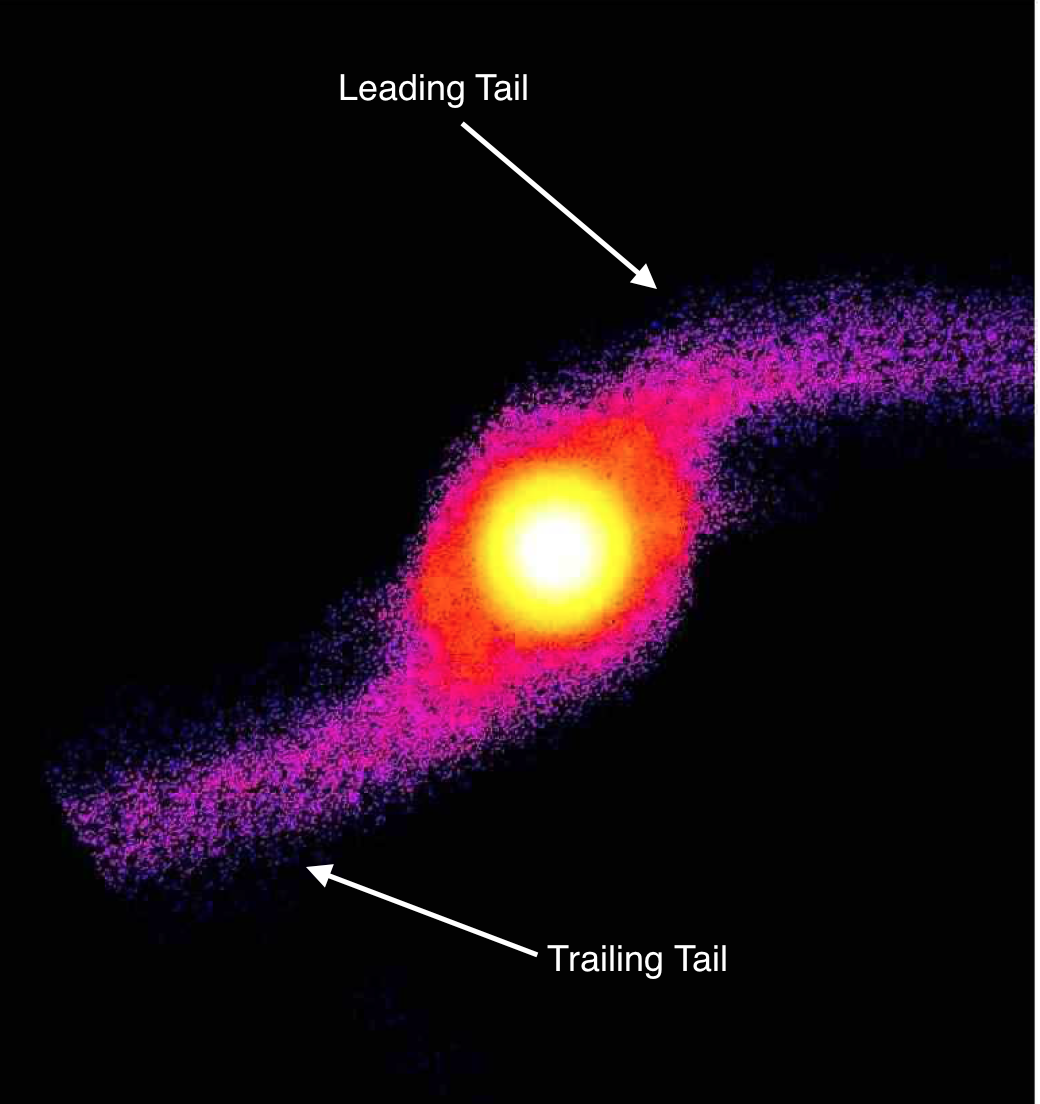
\includegraphics[width=0.5\textwidth]{tailStreams}	
	\caption{The tail streams of a satellite, from Choi et al. (2008)}
	\label{fig:tailstreams}
\end{figure}

In order to test the effectiveness of the simulation, we modeled the Sagittarius satellite on a completely circular orbit, with the exact values shown in table \ref{tab:massTable}.

The satellite and the Milky Way behave as a two-body rotating system. The Milky Way's tidal field adds energy to the orbiting satellite, which in turn drives mass loss from the satellite, a combination of the forces from the Milky Way and the non-inertial forces from the satellite orbit (\cite{structureofDarkMatterHalos}). In this system, test particles (e.g. stars) pass through the two Lagrange points (L4 and L5), which results in the test particles escaping at these points. As a result of the escape, the two Lagrange points define a constantly changing tidal radius, since the Lagrange points are where the radial forces are balanced, as found by \cite{dynamicsOfTidalTails}. This results in the two-tailed system of stellar streams.

To exactly create the two-tailed system, it must be clear what forces are acting on the escaped stars. Stars stripped by tidal forces through the outer Lagrange points move to higher energy orbits with longer periods, resulting in their deceleration, eventually forming the trailing tail. On the other hand, stars stripped through the inner Lagrange point accelerate, as a result of moving into a lower energy orbit with shorter periods. Because of the two distinct tidal iteractions, \cite{ibataLewis} found that the acceleration of the frontal stars and deceleration of the trailing stars results in two striking tails, shown in figure \ref{fig:tailstreams}.

Since the satellite disruption is an effect on the gravitational field of the satellite past the tidal radius, we used the Sagittarius satellite in the first circular orbit. Here, the expectation is that the majority of the mass within the satellite becomes unbound near the Lagrange points. With the Sagittarius galaxy starting at $0.4R_{vir}$, and 4 different timestep snapshots at $T$ = 0.0, 1.5, 3.0, and 4.5, we found that the Sagittarius satellite would eventually smear itself across the entire orbit. At 1.5, the satellite displayed signs of stretching itself across the entire lower right quarter of the orbit, while at 3.0 the satellite had created a stream across the entire left half of the orbit. At 4.5, the satellite had almost covered the entire orbit with a stellar stream. 


\section{Results}
\subsection{Satellite Changes}
\begin{figure}
	\centering
	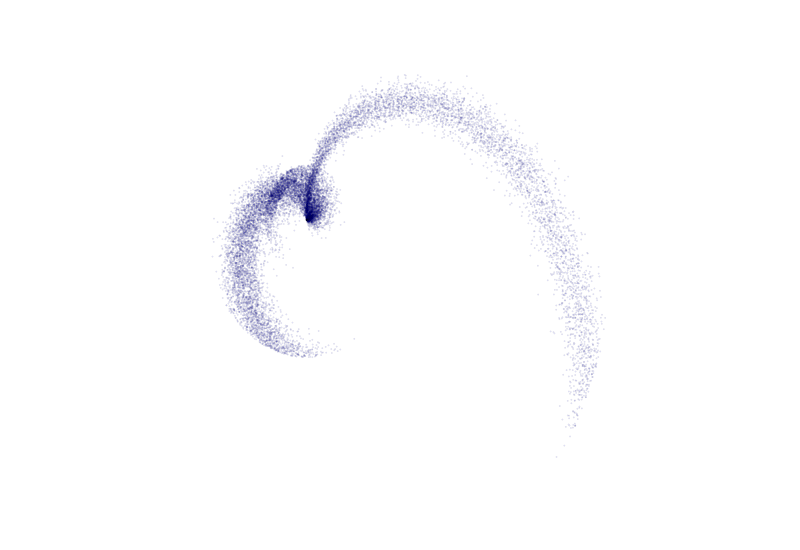
\includegraphics[width=0.5\textwidth]{small.png}	
	\caption{Tail Formation at $T$ = 4.0 for the small satellite. }
	\label{fig:small}
\end{figure}

\begin{figure}
	\centering
	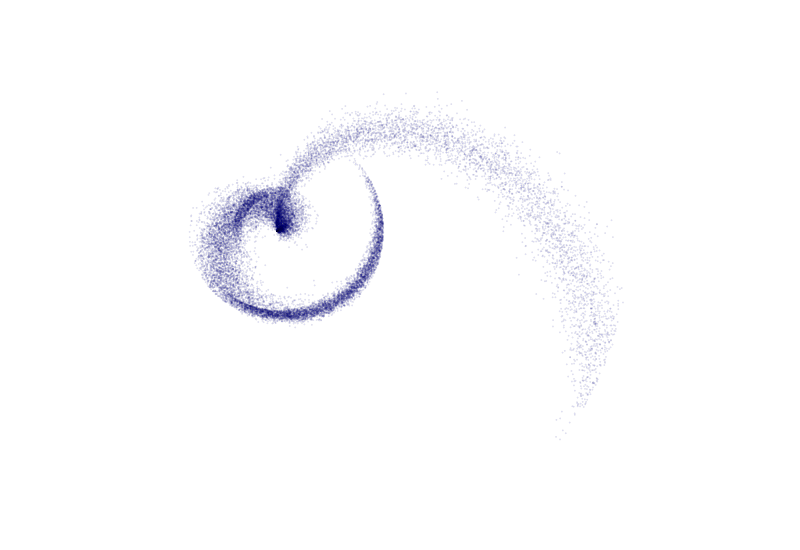
\includegraphics[width=0.5\textwidth]{medium.png}	
	\caption{Tail Formation at $T$ = 4.0 for the Sagittarius-sized satellite. }
	\label{fig:medium}
\end{figure}

\begin{figure}
	\centering
	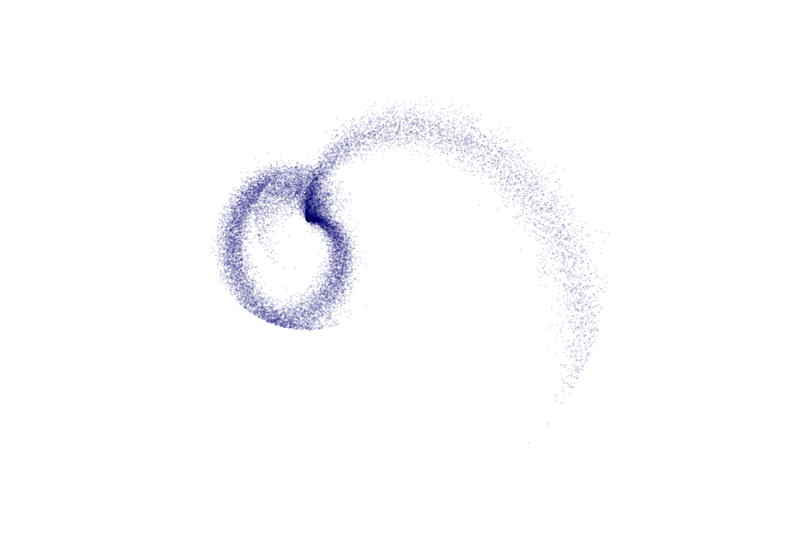
\includegraphics[width=0.5\textwidth]{large.png}	
	\caption{Tail Formation at $T$ = 4.0 for the massive satellite. }
	\label{fig:large}
\end{figure}



Throughout the simulation, 3 different types of satellites around the Milky Way were modeled, described in the table \ref{tab:massTable}.

As the satellite's gravity increases as the mass changes, the stellar streams produced in this interaction would be subject to the same change. By starting out the massive satellite as an isotropic ball of mass and evolving it along a circular orbit with $r = 0.4R_{vir}$, it was found that the satellite produced a stellar stream similarly to initially expected. Originally, it was predicted that the accretion of the stars that escaped through the inner Lagrange point would fall towards the center of the Milky Way, while stars that escaped through the outer Lagrange point would slowly drift away. The simulation found that the satellite produced a stellar stream with two distinctive parts: a leading tail that quickly fell into the center of the Milky Way, and also created a smaller trailing tail. This is extremely similar to the results found by \cite{dynamicsOfTidalTails}, who found that the leading tail tilts towards the center of the halo (akin to the Milky Way used in our simulation), and had a trailing tail that is distributed outside the orbital radius. While the tail modeled by \cite{dynamicsOfTidalTails} started to point directly towards the center of the halo, the tail we found did not, rather only pointing to the center of the satellite. This suggests that possibly more time should be allotted for the simulation, as Choi's leading tail only began to point towards the center at late times, shown in figure \ref{fig:choi_large} In both cases, stars within the leading tail were found to lose energy and angular momentum, resulting in their infall into the Milky Way, whereas the orbits in the trailing tail gained energy and angular momentum, leading to the spread of the trailing tail outside the orbit. This can easily be seen in figures \ref{fig:small}-\ref{fig:large}, which are a position plot of the stars within the stellar stream after two full revolutions. Compare this to figures \ref{fig:choi_small}-\ref{fig:large}, which are the results of \cite{dynamicsOfTidalTails}.

\begin{figure}
	\centering
	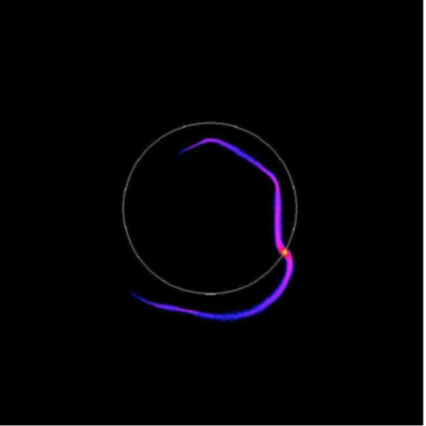
\includegraphics[width=0.5\textwidth]{choi_small.png}	
	\caption{Tail Formation at $T$ = 4.0 for Choi's small satellite. From \cite{dynamicsOfTidalTails}. }
	\label{fig:choi_small}
\end{figure}

\begin{figure}
	\centering
	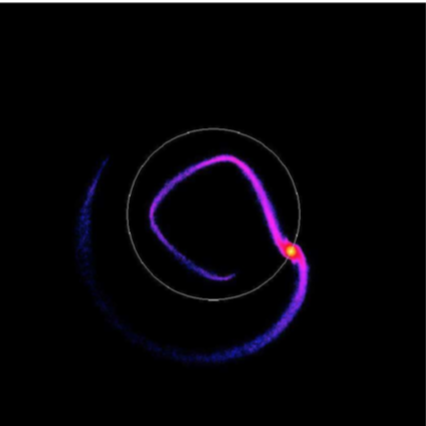
\includegraphics[width=0.5\textwidth]{choi_medium.png}	
	\caption{Tail Formation at $T$ = 4.0 for Choi's Sagittarius-sized satellite. From \cite{dynamicsOfTidalTails}.}
	\label{fig:choi_medium}
\end{figure}

\begin{figure}
	\centering
	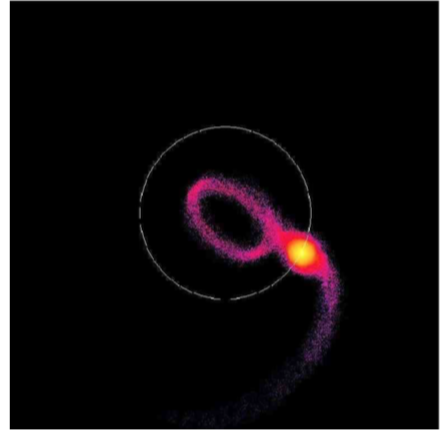
\includegraphics[width=0.5\textwidth]{choi_large.png}	
	\caption{Tail Formation at $T$ = 4.0 for Choi's massive satellite. From \cite{dynamicsOfTidalTails}.}
	\label{fig:choi_large}
\end{figure}

The tail morphology for both the Sagittarius and small sized satellites correspond in the same manner, with the leading tail moving inwards towards the Milky Way and the trailing tail moving outside the orbital radius, eventually becoming smeared along the orbital path. A minor detail in tail morphology for the Sagittarius and small sized satellites is that their tails exhibit major angular shifts in their leading tails. While the large satellite falls changes into a spiral fashion, the Sagittarius and small sized satellites exhibit much sharper kinks instead of curving into the center of the Milky Way. This is explained by \cite{debrisSatellite}, where the sharp kinks in the tails are a result of the cyclic motion alongside the satellite being accelerated at subsequent apocenters. That is, as the satellite continues to orbit, the lingering stellar stream is continually torqued by the remaining satellite. The first sharp turn correlates with the first apocenter of the ejecta, which suggests that the deceleration during escape causes these sharp turns to occur. \cite{binneyTremaine} suggest using a more complex three-body approach to understanding these orbits, using a conserved Jacobi constant with:

\begin{equation}
E_J = E - \Omega^{\rightarrow}_{s}\cdot L^{\rightarrow} 
\label{eq:jacobi}
\end{equation}

where $E$ is the orbital energy, $L^{\rightarrow}$ is the angular momentum, and $\Omega^{\rightarrow}_s$ is the angular frequency of the satellite around the Milky Way. An isocontour of the Jacobi constant passes through the Lagrange points, $r_{L}$, and separates the leading and trailing tails. Since the strength of the tidal forces around the satellite is inversely proportional to the satellite mass (\cite{dynamicsOfTidalTails}), small satellites have a tidal force that is symmetric around the center of the satellite, which then leads to symmetric masses within the leading and trailing tails. In large satellites, however, the asymmetric tidal force means the leading and trailing tails are asymmetric themselves. 

Now we can consider the mass lost through the inner Lagrange point ($r_L$). This orbit will have an inward velocity and unbound values for the Jacobi constant. As a result of this, the force from the satellite continues to affect the orbit beyond the tidal radius, even in the restricted regime of the $N$-body simulations. The smaller the mass of the satellite, the closer the tidal radius is to that of the satellite, which means that the ejected tails then linger near the original satellite orbit. This results in the orbit continuing to be torqued by the satellite, as described by \cite{dynamicsOfTidalTails}.

Figures \ref{fig:smallDist}-\ref{fig:largeDist} show the effect of \ref{eq:jacobi}, showing the distribution of stars with respect to the center of the satellite. Taller bars indicates higher concentration of stars within that angular bin, and higher $\theta_{\parallel}$ values indicate further distance from the center of the satellite. A few noticeable parts are the spikes on the left and right of the center within the small and Sagittarius-sized galaxies, showing that there is a higher concentration of stars within a certain area. This is a result of the kinks leading to a higher concentration of stars within that area, causing a spike in the histogram. 

\begin{figure}
	\centering
	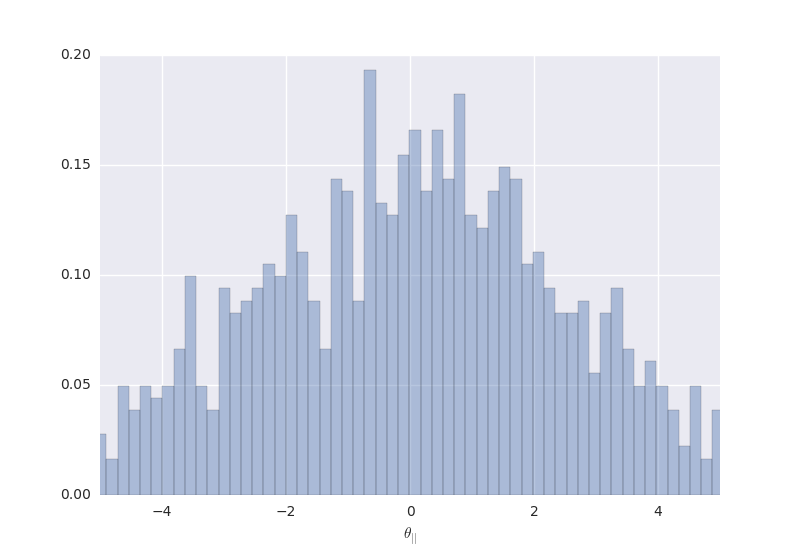
\includegraphics[width=0.5\textwidth]{small_2.png}	
	\caption{Distribution of stars with respect to the center of the small satellite at $T$ = 4.0. }
	\label{fig:smallDist}
\end{figure}

\begin{figure}
	\centering
	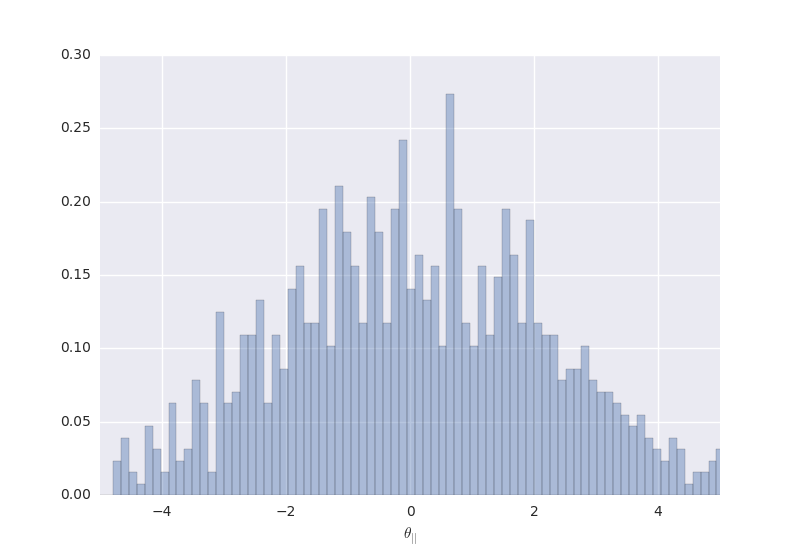
\includegraphics[width=0.5\textwidth]{medium_2.png}	
	\caption{Distribution of stars with respect to the center of the Sagittarius-sized satellite at $T$ = 4.0. }
	\label{fig:mediumDist}
\end{figure}

\begin{figure}
	\centering
	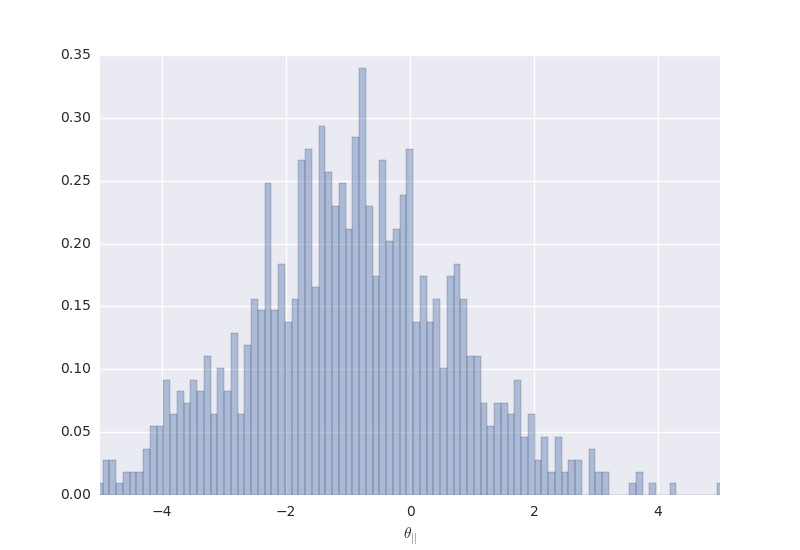
\includegraphics[width=0.5\textwidth]{large_2.png}	
	\caption{Distribution of stars with respect to the center of the large satellite at $T$ = 4.0. }
	\label{fig:largeDist}
\end{figure}

\section{Discussion}
\subsection{Simulation Discussion and Faults}
Both tails shapes have already been previously observed by \cite{grillmairDionatos} and \cite{leonCombes}, which suggests that the simulations carried out are correct representations. However, due to the simplicity of the simulations carried out, the results are not wholly correct. The simulation only takes into account the two theorized dynamical principles that affect stellar stream production demonstrated by \cite{ringsAndPseudoRings}: 1) the leading and trailing points where the attractive force of the host galaxy and the satellite are equal and divergent, leading to a balance with zero velocity at the Lagrange points, and 2) the escaping stars that form the stellar stream are affected differently for the leading and trailing stream, with the leading stream being decelerated and the trailing stream being accelerated from the original orbital spot. \cite{dynamicsOfTidalTails} showed that these two dynamical principles are consistant with the effect of the satellite's self gravitational force on the tail is only weakly related to the satellite's mass, which then means that the acceleration on the satellite after escapes begins to have a significant effect for satellites with masses greater than or equal to the mass of the Sagittarius galaxy. 

Due to this, the simulations imply that any satellite will create a stellar stream that is displaced from the original orbital position. The direction, shape, and magnitude of displacement are all related to the progenitor satellite mass, with higher mass progenitor satellites causing thicker and less tightly bound stellar streams, shown in figures \ref{fig:small}-\ref{fig:large}. The distance in which the leading tail travels is also shown to be a result of the progenitor mass, with higher progenitor masses causing a smaller orbital radius for the leading tail and lower progenitor masses causing a larger orbital radius. Figures \ref{fig:smallDist}-\ref{fig:largeDist}, along with \ref{eq:jacobi} show that orbital kinks are a direct result of progenitor masses. 

To complete the simulation, there were some major assumptions made about the initial conditions. First, the effects of dynamical friction were completely ignored, as \cite{dynamicalFriction} found that dynamical friction was only relevant on a star's nearest neighbors, which means that the neglect of dynamical friction would only affect a very small subset of stars. Second, the Milky Way halo was modeled to be completely isotropic and spherical, which affected the models of the satellites. Since the satellites were shifted into orbit according to tidal forces, a non-spherical Milky Way halo would pull satellite shapes away from being a completely isotropic sphere. For the purposes of the simulation however, a spherical Milky Way halo and satellite serve as good control values. Third, the satellite was assumed to be on a circular orbit around the Milky Way well within the tidal disruption radius of the Milky Way. If eccentricity was introduced into the orbit of the satellite, the stellar stream created would exhibit velocity distributions with far more disparities, leading to more varied results and a larger leading/trailing tail split. However, \cite{dynamicalFriction} found that this eccentricity is only important for satellites and dark matter halos of modest mass, meaning that the simulation is roughly accurate for the small and Sagittarius sized satellites. Finally, the assumption was made that the Milky Way halo remains spherically isotropic despite interactions with the satellite, that is, only the satellite would create the stellar stream. Properly speaking, stars from the Milky Way would also be pulled out of orbit in order to create the stellar stream, but those stars are far less numerous than the stars from the satellite, thus leading us to neglect them from our calculations. 

\subsection{Further Experimentation}

A variety of further experimentation can be conducted on stellar streams. This paper neglected the processes of eccentricity within orbits completely, which means that more trials could be conducted on eccentric orbits, such as the orbits of NGC-4651, or orbits following the bifurcation of the Sagittarius stream. Another addition could be to model satellite galaxies in a non-spherical fashion, as this paper neglected the processes of the Milky Way disk and satellite disks. 



\bibliography{finalPaper} 

\end{document}